\section{Problem formulation: unsupervised embedding translation}

Consider a collection of embedding vectors $\{u_1, \ldots u_n\}$, for example, a dump of a compromised vector database, where each $u_i = M_1(d_i)$ is generated by an unknown encoder $M_1 : \mathbb{V}^s \rightarrow \R^{d_{M_1}}$ from an unknown document $d_i$.  We cannot make queries to $M_1$ and do not know its training data, nor architectural details.  Our goal is to extract any information about the documents $d_i$.

% The only available information is the cosine similarities between vectors, i.e., the embedding geometry.  


\begin{figure}[t]
    \centering
    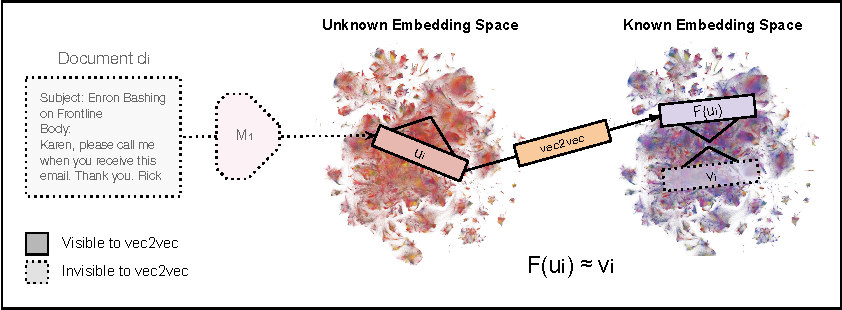
\includegraphics[width=0.9\linewidth]{ims/spaces.pdf}
    \caption{\textbf{Unsupervised embedding translation}. With access to only $u_i = M_1(d_i)$, \atk{} seeks to generate a translation $F(u_i)$ that is close in $M_2$'s embedding space to the ideal embedding $v_i = M_2(d_i)$ without access to $d_i$, $v_i$, $M_1$, or $M_2$.}
    % https://docs.google.com/drawings/d/15lO_xIOkSc-jI75ThhHp4K_mFUQFW0nI--rZyht2avg/edit?usp=sharing
    \label{fig:spaces}
\end{figure}

We do assume access to a different encoder $M_2$ that we can query at will to generate new embeddings in some other space.  We also assume high-level distributional knowledge about the hidden documents: their modality (text) and language (e.g., English).  To extract information, we may translate $\{u_1, \ldots u_n\}$ into the output space of $M_2$ and apply techniques like inversion that take advantage of the encoder.

\shortpara{Correspondence methods cannot be used.}
There is significant prior research on the problem of \textit{matching} or \textit{correspondence} between sets of embedding vectors \citep{alvarezmelis2018gromovwassersteinalignmentwordembedding, peyre2016gromov, chen2020graphoptimaltransportcrossdomain, schnaus2025itsblindmatchvisionlanguage}.  None of these approaches are applicable in our setting because they assume the existence of two (or more) sets of embedding vectors produced by different encoders from the \emph{same inputs}.  In other words, for each unknown vector, there must already exist a set of candidate vectors in a different embedding, one of which is the correct match. In practice, it is unrealistic to expect that such a database be available.
\footnote{Our code is available \href{https://github.com/rjha18/vec2vec/}{on GitHub.}}


% The correspondence setting is a good testbed and idealized baseline for new methods, but it is unrealistic in practical scenarios, such as recovering information from a vector database without access to the encoder.  Even unsupervised matching \citep{schnaus2025itsblindmatchvisionlanguage} can only identify a document's index in the database if they are given a different embedding database with the same documents. In practice, it is unrealistic to expect that such a database be available.



% \paragraph{Translation is strictly harder.}

In our setting, where we do not assume access to the encoder $M_1$, nor any additional representations of the unknown documents $\{d_1, \ldots, d_n\}$ other than their embeddings $u_i=M_1(d_i)$, the problem is strictly harder and requires unsupervised \textit{translation} from $M_1$ to $M_2$. 
Any success at unsupervised translation will come solely from the common geometric structure of $M_1$'s and $M_2$'s output spaces.

\shortpara{The Strong Platonic Representation Hypothesis.} 
Our hope that unsupervised embedding translation is possible at all rests on the stronger version of the Platonic Representation Hypothesis \citep{huh2024platonicrepresentationhypothesis}.  Our conjecture is as follows:
\emph{neural networks trained with the same objective and modality, but with different data and model architectures, converge to a universal latent space such that a translation between their respective representations can learned without any pairwise correspondence.} 

% The success of any unsupervised translation method would provide preliminary evidence to support this hypothesis. \rj{'mapping'}


\shortpara{Translation enables information extraction.} Solving unsupervised translation will allow us to use information extraction tools designed to operate on vectors produced by known encoders. For example, we could apply inversion models \citep{morris2023textembeddingsrevealalmost, zhang2025universalzeroshotembeddinginversion} to recover unknown documents $\{d_i\}$.

% the hidden documents referenced in the database. The amount of information extracted is highly dependent on translation quality, since reliable information extraction from embeddings necessitates high-fidelity reconstructions of the embeddings themselves \citep{morris2023textembeddingsrevealalmost}.
